%TCIDATA{LaTeXparent=0,0,relatorio.tex}



\chapter{Análise de Dados} \label{chap:Resultados}

% Resumo opcional. Comentar se não usar.
\resumodocapitulo{``Analisar os dados tops!'' -- Tiago}


\section{Introdução}

Nesse capítulo iremos explicar um pouco melhor os experimentos realizados, descritos na seção \ref{section:TestesRealizados}. Iremos também mostrar seus resultados e analisá-los. Lembrando que os experimentos realizados foram:

\begin{itemize}
	\item Apendizagem de 3 comportamentos em um mapa pequeno
	\item Apendizagem de 3 comportamentos no mapa clássico
	\item Apendizagem de 5 comportamentos em um mapa pequeno
	\item Apendizagem de 5 comportamentos no mapa clássico
\end{itemize}

\section{3 Comportamentos no mapa pequeno}

Nesse experimento%
\footnote{Os parâmetros e o setup desse experimento estão melhor descritos no tópico \ref{subsection:3ComportamentosMapaPequeno}.%
} utilizamos apenas 3 comportamentos, $ B = \{Ficar\_Parado, Comer, Fugir\} $, e usamos como vetor de características $ f $, sendo ele:

\begin{equation}
	\begin{array}{l}
		f_1 \left( a, u \right) = 1.0 \\
		f_2 \left( a, u \right) = ObterCaracteristicaDistanciaComida \left( a \right) \\
		f_3 \left( a, u \right) = ObterCaracteristicaProbFantasmas \left( a \right)
	\end{array}
\end{equation}

Realizamos o treinamento ao longo de 2700 partidas, sendo que a exploração gulosa (\textit{greedy exploration}) foi executada até a partida 1500. Após terminado o treinamento utilizamos 300 partidas para avaliar e obter dados sobre o algoritmo treinado.


\subsection{Resultados e Análise}

A evolução da aprendizagem se dá a partir da mudança dos pesos $ \omega_i $ ao longo do tempo, devido à sua relação com o comportamento selecionado via a equaçào \ref{equation:QLearningEscolhaComportamentoFinal}. Nas figuras \ref{img:3ComportamentosMapaPequeno:PesoBias}, \ref{img:3ComportamentosMapaPequeno:PesoDistComida}, \ref{img:3ComportamentosMapaPequeno:PesoProbFantasma} temos os gráficos de como os valores desses pesos evoluem com o tempo, para cada um dos comportamentos.

\begin{figure}[H]
    \centering
    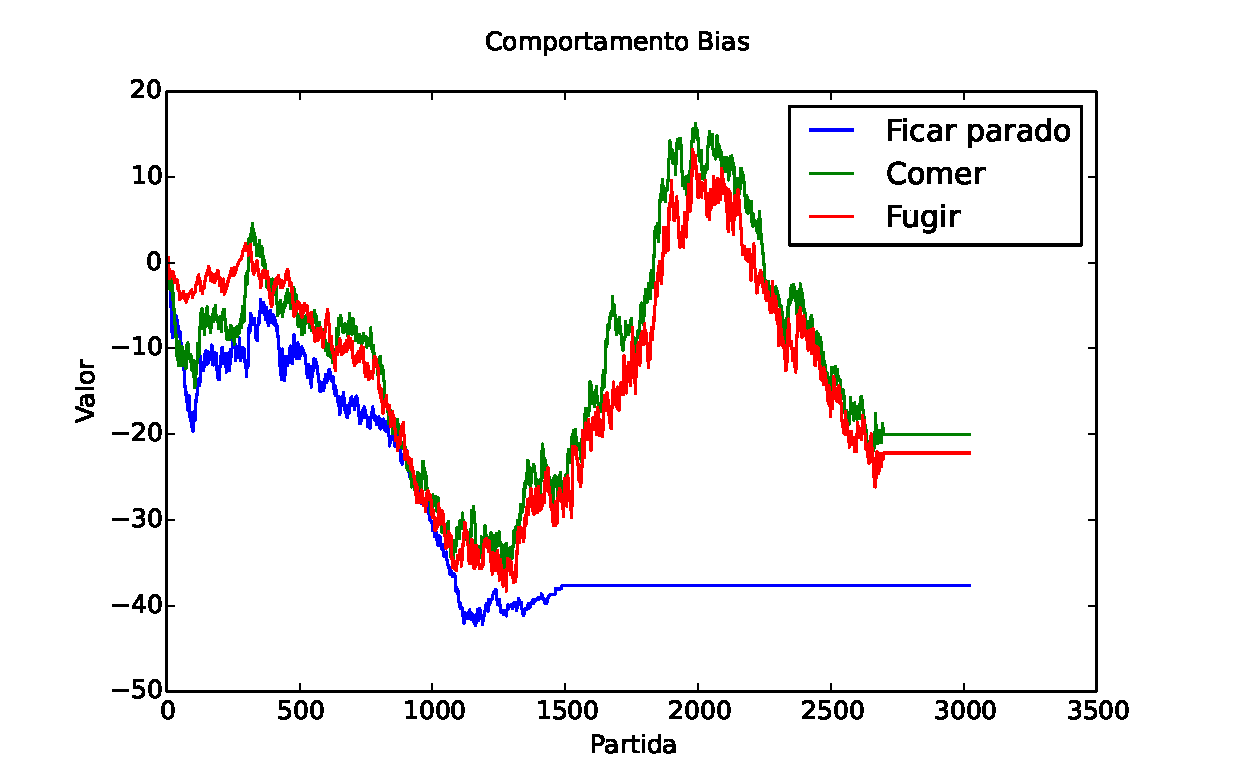
\includegraphics[width=\linewidth]{images/3_behaviors_small_map/weights____pol__Bias}
    \caption{Evolução dos pesos $ \omega_1 $ da característica Bias $ f_1 $.}
    \label{img:3ComportamentosMapaPequeno:PesoBias}
\end{figure}

\begin{figure}[H]
    \centering
    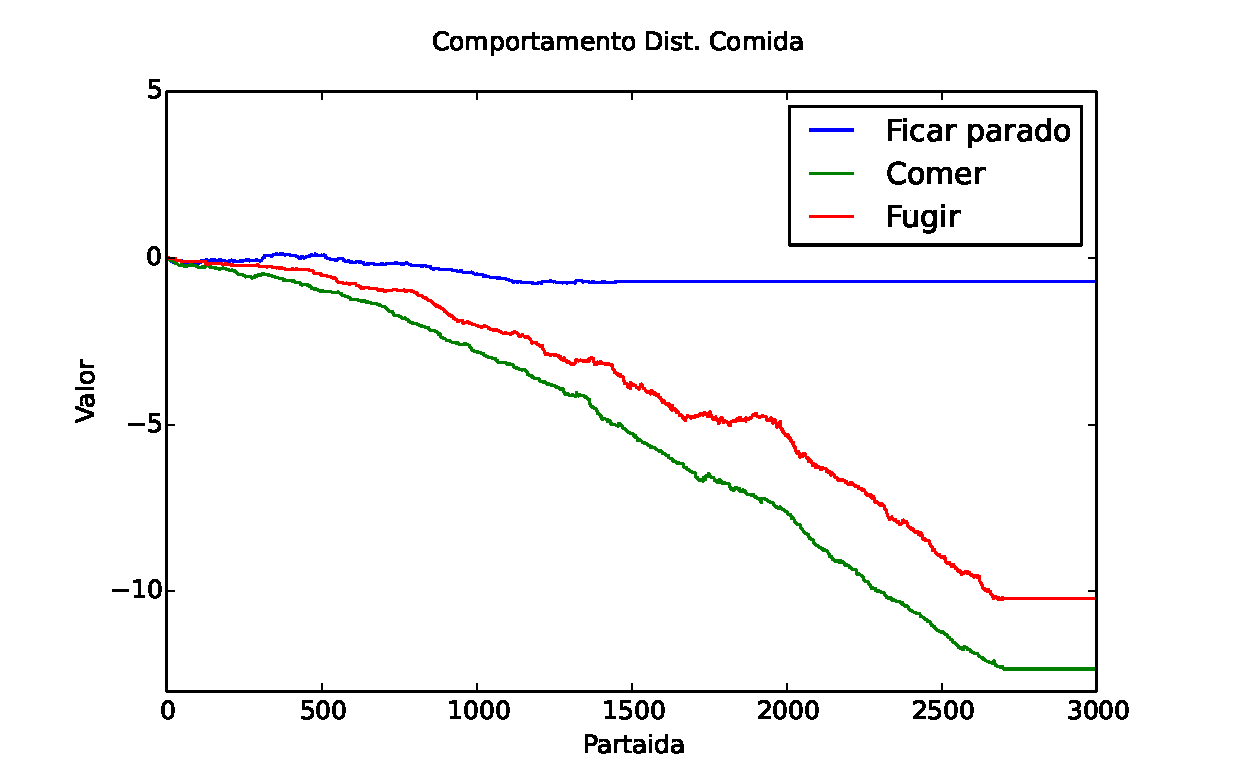
\includegraphics[width=\linewidth]{images/3_behaviors_small_map/weights____pol__DistComida}
    \caption{Evolução dos pesos $ \omega_2 $ da característica Distância para Comida $ f_2 $.}
    \label{img:3ComportamentosMapaPequeno:PesoDistComida}
\end{figure}

\begin{figure}[H]
    \centering
    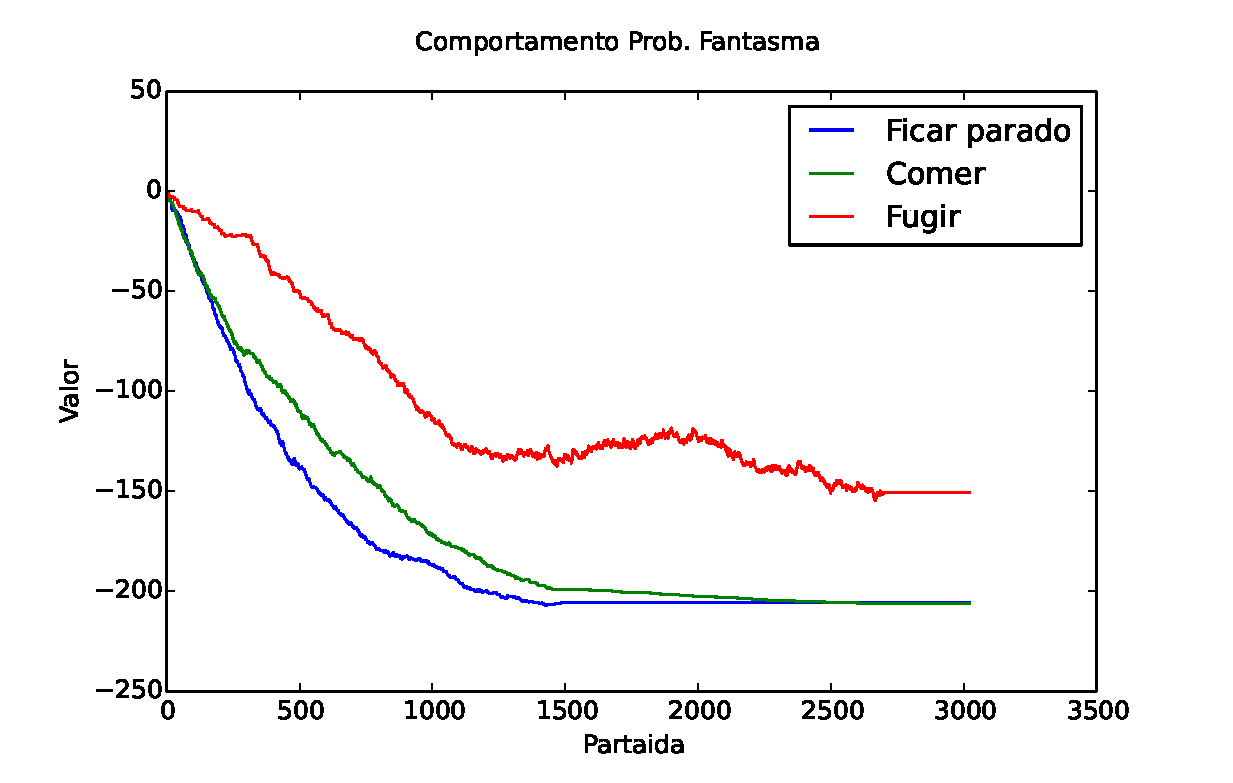
\includegraphics[width=\linewidth]{images/3_behaviors_small_map/weights____pol__ProbFantasma}
    \caption{Evolução dos pesos $ \omega_3 $ da característica Probabilidade de Fantasma $ f_3 $.}
    \label{img:3ComportamentosMapaPequeno:PesoProbFantasma}
\end{figure}


Outro fator importante nesse algoritmo é qual comportamento foi escolhido a cada instante, e quantas vezes cada um é escolhido por partida. Quando pegamos o número de vezes que cada comportamentos é escolhido por partida e plotamos esses dados como pontos num gráfico eles formam a seguinte nuvem, exposta na figura \ref{img:3ComportamentosMapaPequeno:ComportamentosEscolhidos}.

\begin{figure}[H]
    \centering
    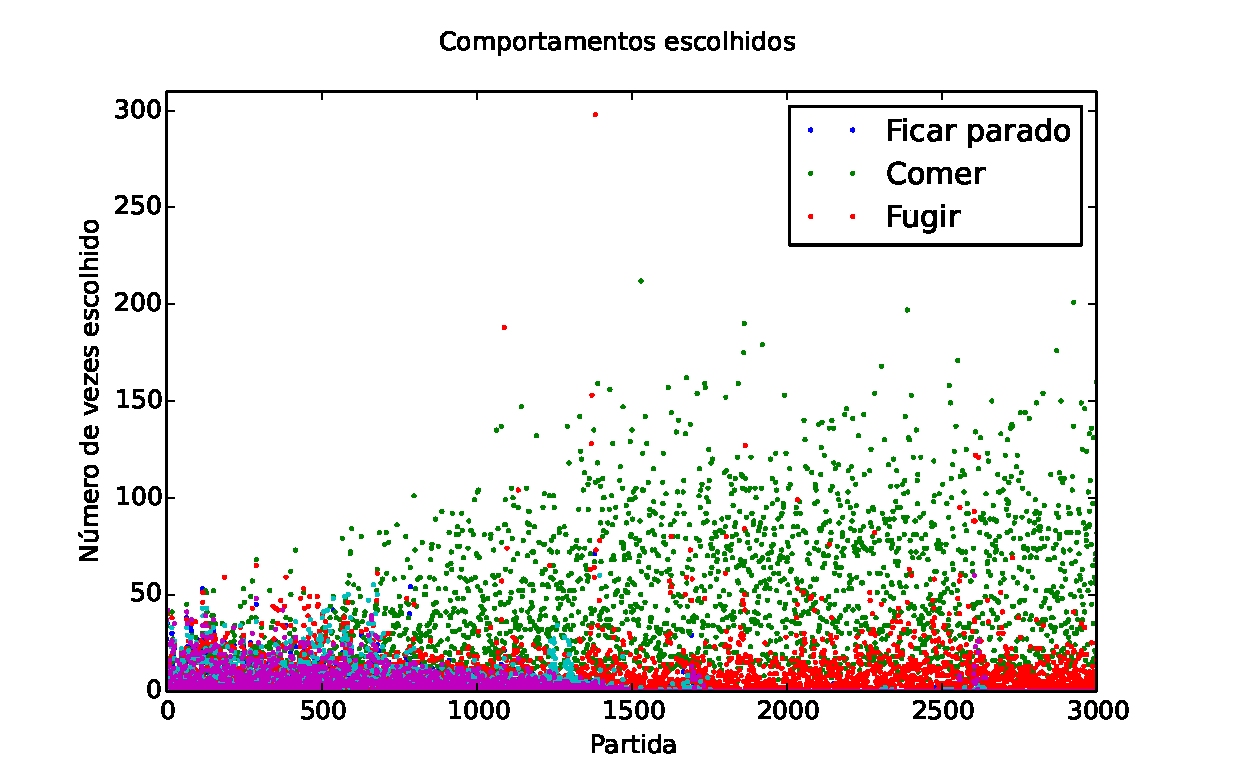
\includegraphics[width=\linewidth]{images/3_behaviors_small_map/chosen_behaviors}
    \caption{Escolha de comportamentos por partida.}
    \label{img:3ComportamentosMapaPequeno:ComportamentosEscolhidos}
\end{figure}

Podemos agora tentar aproximar um polinômio dessa nuvem de pontos, utilizando o método dos mínimos quadrados. Para um polinômio de quarto grau essa curva fica como a descrita na figura \ref{img:3ComportamentosMapaPequeno:ComportamentosEscolhidosPolinômio}.

\begin{figure}[H]
    \centering
    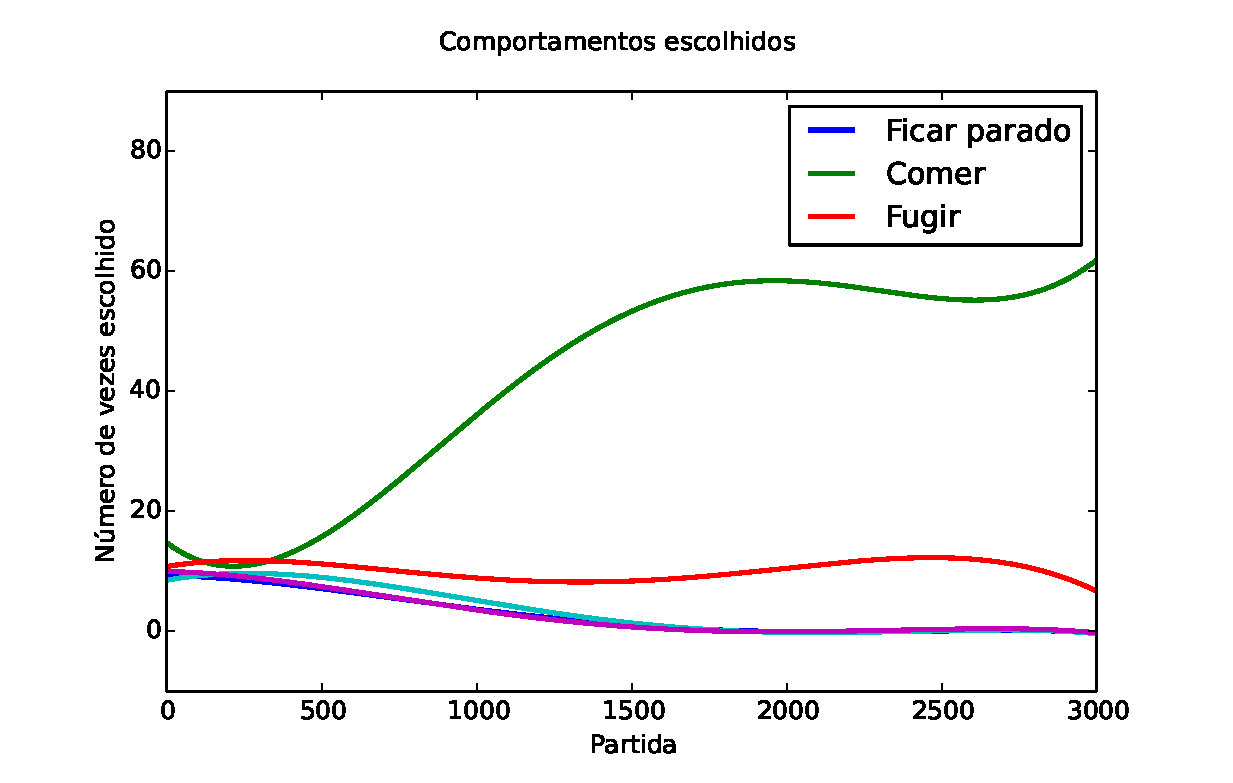
\includegraphics[width=\linewidth]{images/3_behaviors_small_map/chosen_behaviors_pol}
    \caption{Escolha de comportamentos por partida.}
    \label{img:3ComportamentosMapaPequeno:ComportamentosEscolhidosPolinômio}
\end{figure}

Outro dado relevante para a análise é a pontuação obtida por jogo, que, como é o que damos como recompensa para nossa função de treinamento, é o que tentamos otimizar. A pontuação para cada partida pode ser vista na imagem \ref{img:3ComportamentosMapaPequeno:PontuacaoPorPartida}, à seguir. Assim como para a evolução dos comportamentos escolhidos ao longo do tempo, também aproximamos esses dados por um polinômio de quarto grau, utilizando o método dos mínimos quadrado.

\begin{figure}[H]
    \centering
    \includegraphics[width=\linewidth]{images/3_behaviors_small_map/match_scores____pol}
    \caption{Escolha de comportamentos por partida.}
    \label{img:3ComportamentosMapaPequeno:PontuacaoPorPartida}
\end{figure}


\subsection{Discussão}



\section{3 Comportamentos no mapa original (Teste 2)}
\section{5 Comportamentos no mapa pequeno (Teste 3)}
\section{5 Comportamentos no mapa original (Teste 4)}
